For robots to become widely accessible, users have to be able to command them by specifying high-level behaviors, not by programming low-level robot controllers.
This has recently become possible by applying tools and ideas from the formal methods and hybrid systems to robotics. The resulting methodologies translate high-level tasks to discrete and subsequently low-level continuous controllers in a correct-by-contstruction manner \cite{BBEFKP06}.
\emph{Reactive} approaches are of particular interest, since they account for a dynamic, and possibly adversarial, environment. For example, the framework in \cite{KGFP_TRO09} takes a logic formula that contains the mission specification and, by solving a two-player game between the robot and its environment \cite{piterman_06}, outputs a hybrid controller that is guaranteed to accomplish the mission. Other reactive approaches have been proposed, e.g., \cite{Wongpiromsarn2010} and \cite{Belta2013RSS}.

However, the initial approaches operate under the closed world assumption, whereas robots have moved from the reclusive workspace of the assembly line to the highly unstructured site of the Fukushima Daiichi nuclear disaster. 
%Thus, there is a need for high-level robot controllers that adapt to the discrepancies between the robot's model of the world and reality. 
In addition, robots are also asked to incorporate new functions during execution. 
Examples include reconfigurable modular robots, as well as robots that learn on-the-fly \cite{SaxenaIJRR2012} or inquire online knowledge repositories \cite{rapyuta2013}. 
Finally, the world may be open with respect to (w.r.t.) goals added after the robot has been deployed, as in the case of robotic search and rescue tasks \cite{MatthiasAI2010}, military scenarios \cite{gda2013}, and autonomous space and planetary exploration missions \cite{spaceXplore2006}. 
%Uncertainty and partial a priori knowledge are inherent aspects of future robot missions, not problems that we should attempt to avoid encountering.

\begin{myExample}\label{Ex:mailbot1}
%For example, consider 
Consider a robotic courier (mailbot; see Fig. \ref{Fig:mailbot}) deployed in a school or company building. 
Its task is to collect letters and deliver them to the recipients' offices. 
This mission is relatively simple, and yet the robot's world is already open w.r.t. letters addressed to recipients that the robot does not know about. % Na to kana entelws nia-nia dew?
Even if all possible recipients, and the locations of their offices, are fixed, the information may not be available a priori.
\end{myExample}
%\begin{myExample}\label{Ex:mailbot1} Autonomous Mailbot (Fig. \ref{Fig:pr3})\\
%	A robotic courier (mailbot) operates within a school or company building. It is tasked with collecting letters and delivering them to the recipients' offices. Even if all possible recipients, and the locations of their offices, are fixed, the information may not be available at the time the mission specification is defined.
%\end{myExample}

\begin{figure}[ht]
	\centering
	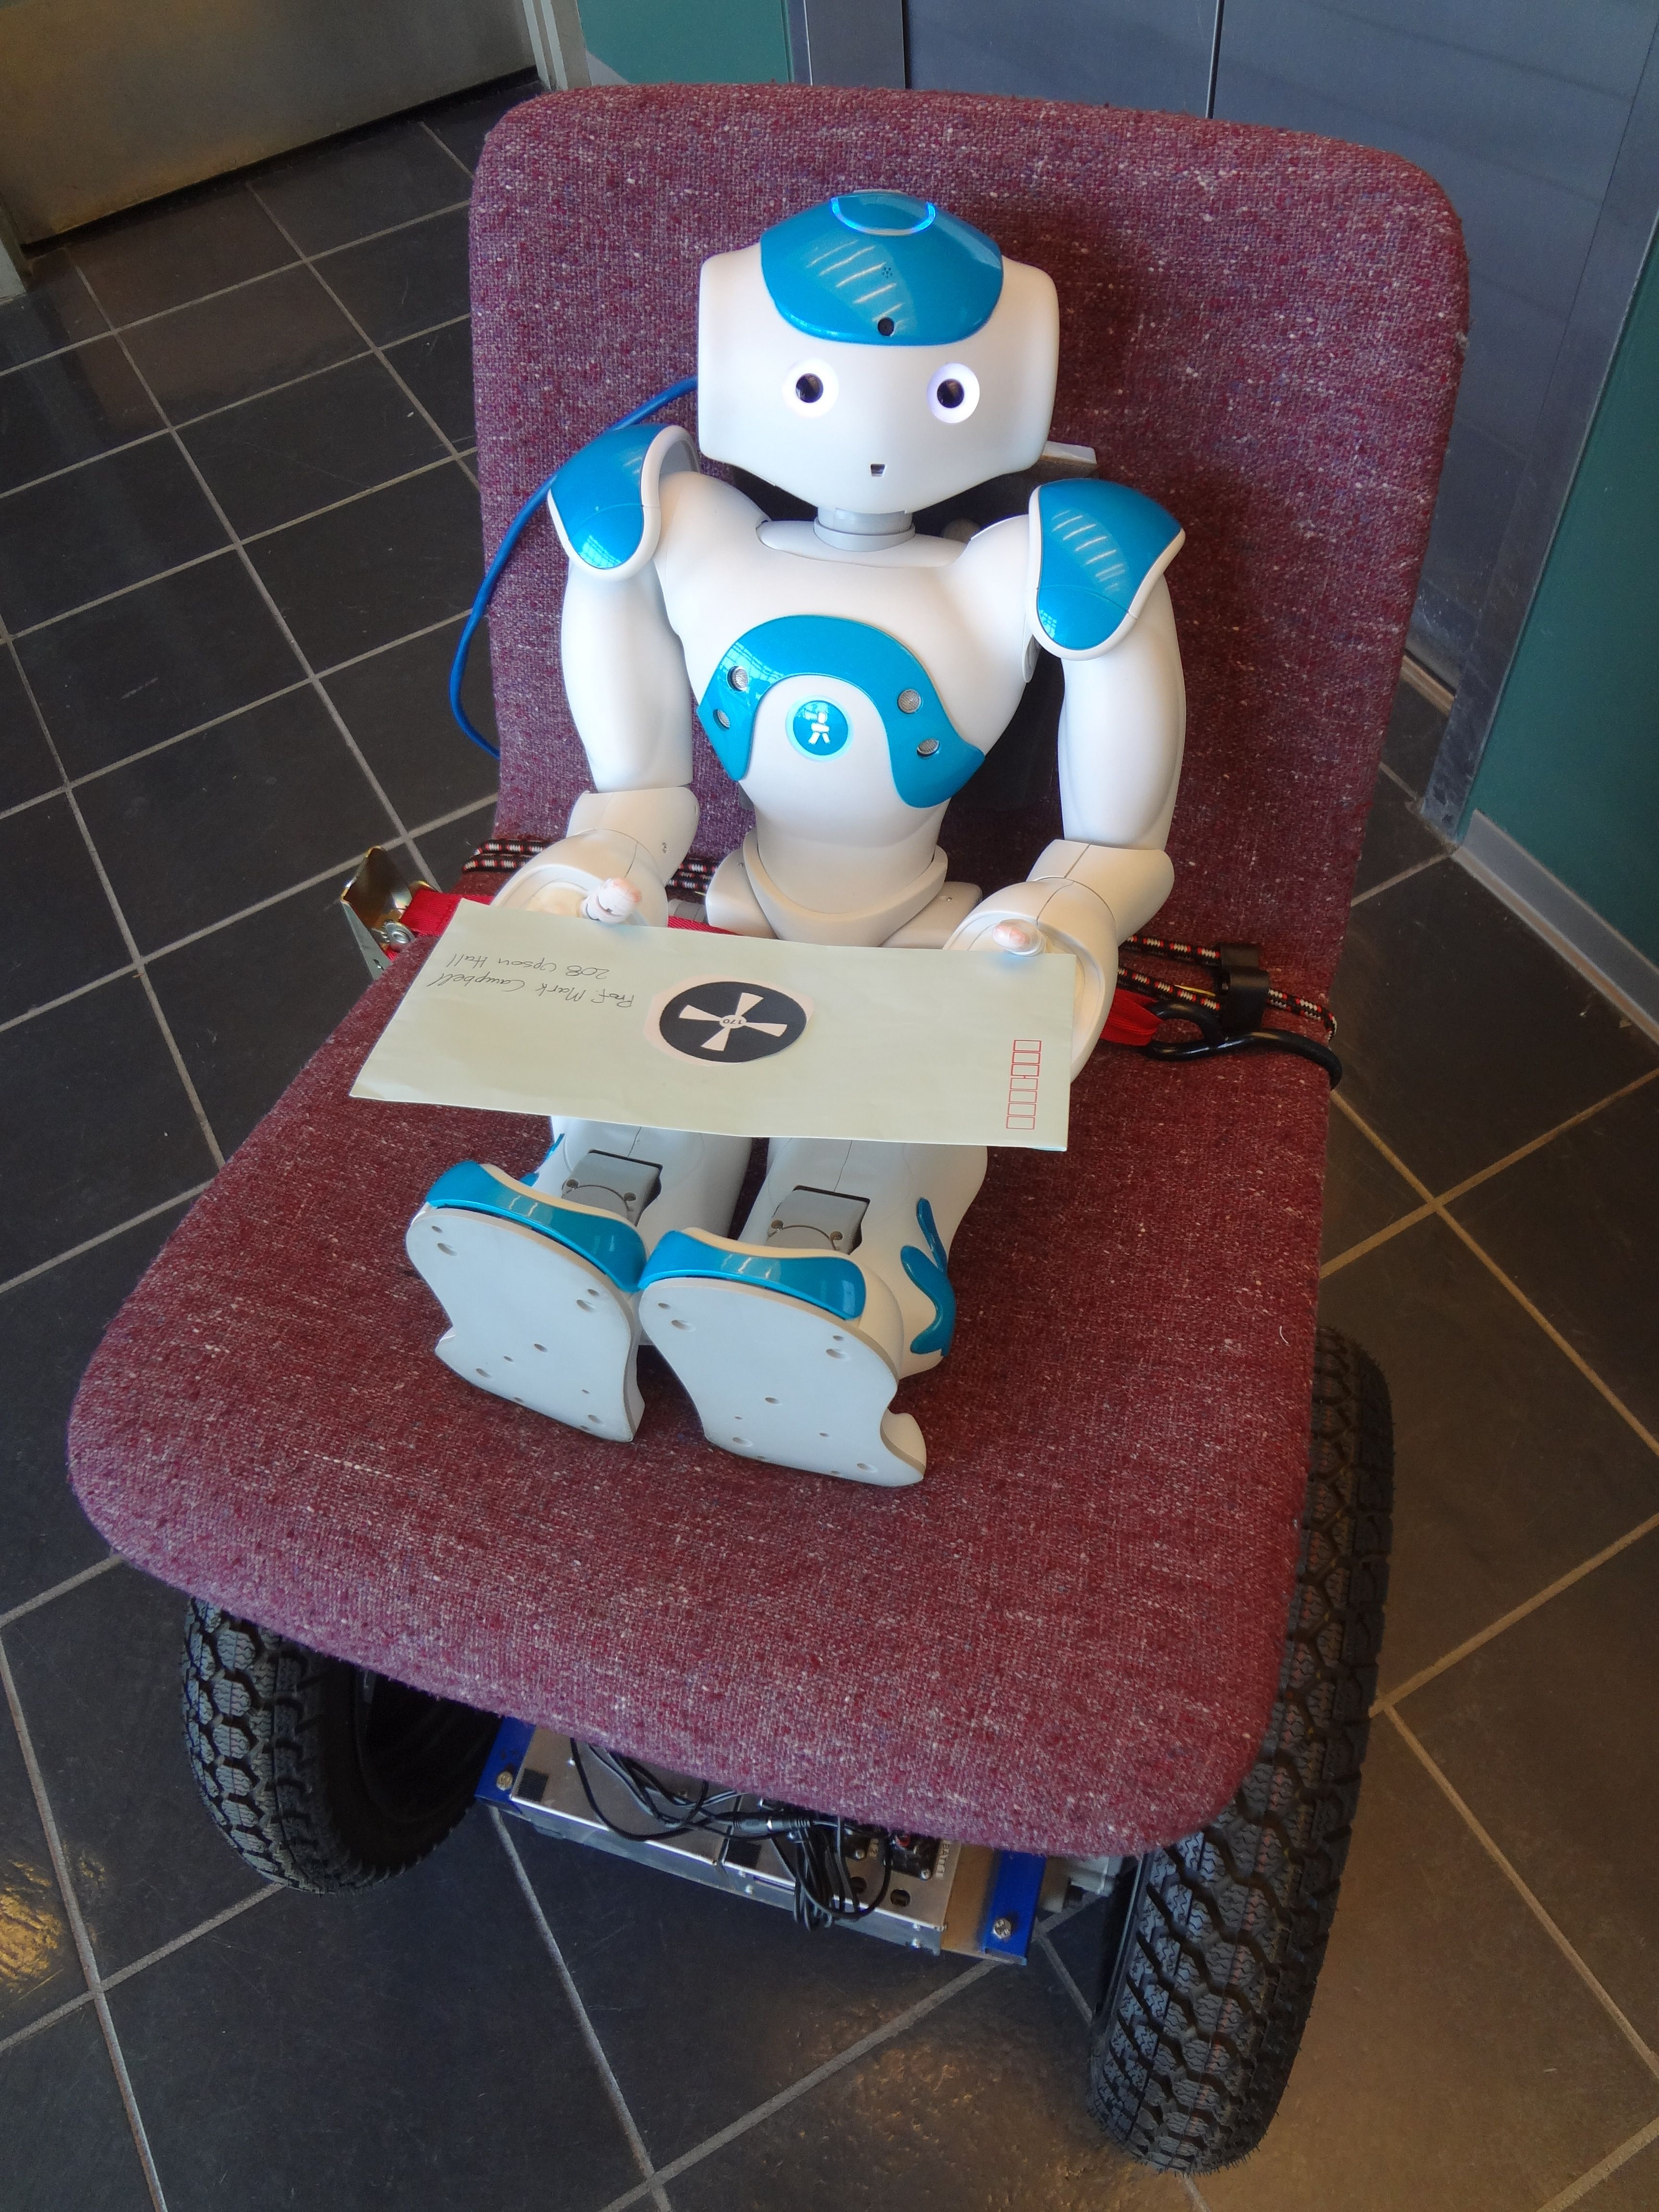
\includegraphics[width=0.7\columnwidth, clip]{./img/mailbot.jpg}
	\caption{Our implementation of a mailbot. A Nao humanoid robot is mounted on a segway platform that includes a lidar sensor. The actuation and perception capabilities of the former are complemented by the localization, navigation and mobility advantages of the latter.}
	\label{Fig:mailbot}
\end{figure}

In order to obtain controllers for worlds open w.r.t new elements, a number of challenges have to be overcome. 
First, there is the assumption that a robot has full knowledge of the structure of its workspace. This issue has been tackled in \cite{MurrayICRA2012} and \cite{MurrayICRA2013a}, where the authors introduced local re-synthesis as a way to account for local topological changes in the robot's workspace. 
An approach that addresses the unreactive equivalent of the same problem appeared in \cite{Dimos2013ICRA}. 
Furthermore, the aforementioned approaches assume that the size of the workspace is known; that only its internal structure changes. In addition, they do not account for augmenting the mission with additional objectives, a situation that may arise if the robot can discover new regions or objects of interest. 
The work in \cite{BingxinRSS2012} allows the robot's workspace to expand, but does not account for the discovery of non-spatial aspects of the world, such as learning new actions or responding to unexpected events.
%A true open world planner must be able to adapt to changes in other parts of the robot's world model as well, such as available sensors and actions. 
Finally, there is the the challenge of specifying open world missions in the first place, since the world is only partially known prior to execution. The specification language and abstractions necessary for this have been approached with both semantic \cite{Joshi2012, MatthiasAI2010} and statistical \cite{Tellex2011} methods, but so far no solution provides the guarantees on behavior that a formal, correct-by-construction system is capable of. 

In this paper, we first propose an approach to writing high-level missions such that the robot's tasks are not specified only in terms of elements in the world that are known prior to execution. This is accomplished via \emph{open world abstractions}, which allow us to specify behaviors implicitly. 
Furthermore, they allow the specification to be updated as new elements of interest are discovered. The new elements include, but are not limited to, the sensing of a new objects and events, and the discovery of new regions of the workspace. They may also lead to new mission goals.
Finally, we show how the mission specification can be systematically and automatically rewritten in order to correctly incorporate these new elements of the open world. 

The paper is organized as follows: Section \ref{preliminaries} provides the necessary background on logic-based reactive mission planning. Section \ref{problem} states the problem. The proposed abstractions, which we will use to specify tasks over open worlds, are treated in Section \ref{abstractions}. Section \ref{openworld} presents our approach to systematically rewriting the mission specification. Simulations of the mailbot scenario (Example \ref{Ex:mailbot1}), which is revisited throughout the paper, are provided in Section \ref{simulation}. Finally, our conclusions, as well as possible research directions, are summarized in Section \ref{conclusion}.

% END